\section{Electromyography}

The control of a myoelectric prosthesis is based on recorded myoelectric signals. \cite{Geethanjali2016}  Enabling the use of myoelectric signals for control of functional prosthetics requires a theoretical background knowledge of the signals origin and how it can be acquired. The following section will describe myoelectric signals and how they are acquired through the acquisition method of electromyography (EMG).   \\
The process of executing a voluntary movement can be explained through electric potentials and the excitability of skeletal muscle fibers. The nerve impulse carrying excitation information of a voluntary muscle contraction will travel from the motor cortex down the spinal cord to a alpha motor neuron. The alpha motor neuron will activate and direct an nerve impulse along its axon to multiple motor endplates, which each innervate a muscle fiber. The motor neuron and the muscle fibers it innervates is in collection called a motor unit. \cite{Turker2013} \\
The nerve impulse initiates the release of neurotransmitters forming an endplate potential. The muscle fibers consist of muscle cells, which each are surrounded by a semi-permeable membrane. The resting potential over the membrane is held at a equilibrium, typically at -80 mV to -90 mV, by ion pumps, which passively and actively control the flow of ions through the membrane. The release of neurotransmitters affects the flow through the ion pumps resulting in a greater influx of Na$^+$. This results in a depolarization of the cell membrane. However, only if the influx of Na$^+$ is great enough to create a depolarization surpassing a certain threshold, an action potential is formed. The action potential is characterized by the cell membrane potential, which changes from around -80 mV to +30 mV. %After the depolarization a repolarization phase occurs and is followed by a hyperpolatization period, restoring the resting potential. 
The created action potential will propagate in both directions on the surface of the muscle fiber. This process happens across all muscle fibers in a motor unit. The action potential is also known as a motor unit action potential (MUAP), and it is the superposition of multiple MUAPs that is recorded through surface EMG. The action potential is still measurable on the skin surface, however, some limitations in surface EMG are that the recording is restricted to superficial muscles, that the amplitude of the EMG signal is affected by the depth of subcutaneous tissue and that the distinguishability of MUAP's from adjacent muscles is unreliable. \cite{Turker2013,Martini2012} \\
Acquisition of EMG-signal can either be carried out through surface EMG or intramuscular EMG. The latter measures MUAPs through needles inserted into the muscle and can and collect MUAPs from single muscle fibers individually. Surface EMG is acquired through electrodes on the skin surface. \cite{Cram2012}  Using surface EMG requires preparation of the skin surface to minimize impedance and maximize skin contact. Hence, the skin should be clean and dry before electrode placement. To further minimize skin-electrode impedance removal of excess body hair or flaky skin and cleansing the area using alcohol swabs should be considered. \cite{Turker2013,Cram2012} In this project MUAPs will be recorded through surface EMG. An example of a surface EMG recording of two different movements (pronation and supination of the wrist) can be seen in \figref{fig:Emg_rot}. Here, the surface electrodes are placed at the circumference of the forearm of the subject. It can be seen that some electrode channels are more or less active when comparing the two movements. This corresponds to different muscles being more or less contracted depending on which movement that is performed. This enables the recognition of which movement is being performed. A prerequisite for this to work is that the electrode placement must be identical throughout the recording. If not, the activation of the various channels shifts spatially, and the accuracy of the trained recognition system might be decreased.

\begin{figure}[H]                 
	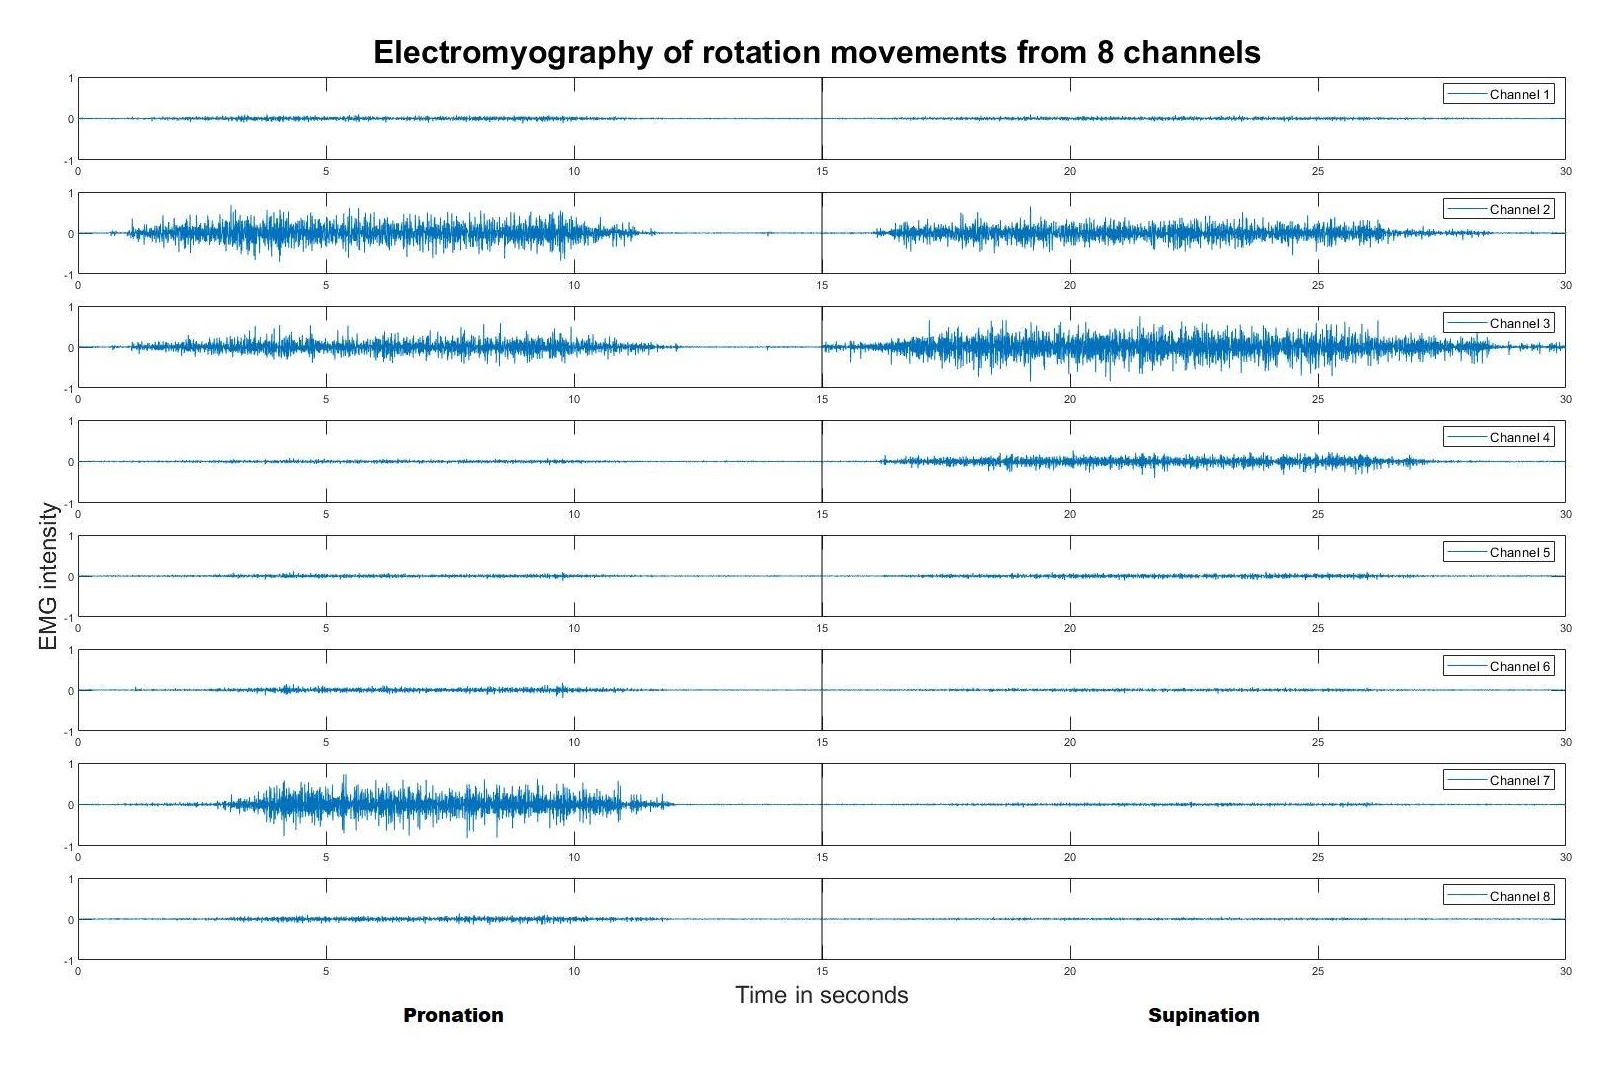
\includegraphics[width=0.95\textwidth]{figures/Emg_rot}  
	\caption{Illustration of an eight electrode channel surface EMG of the forearm during pronation (left side) and supination (right side) of the wrist. The recording was acquired using the Myo Armband, see \figref{fig:MYB}. The 4th channel was placed on the thickest part of the forearm centrally on the anterior side, when using a pronated arm as reference position, with the horizontal LED light faced laterally towards the wrist.}
	\label{fig:Emg_rot} 
\end{figure}

%surface and iemg emg             
